\chapter{Evaluation}

The purpose of this chapter is to explain how the final iteration of the prototype was evaluated. The chapter will focus on the evaluation methods used, as well as representing data and discussing the results. The evaluation aimed towards concluding upon the final problem statement, and provide a better understanding about collaboration in groups.

\section{Methods}
This section will cover which methods that were used in correlation to the methods chapter (insert referance).
\section{The test}
This section will go into detail on how the actual test was conducted, as well as which variables that were to be considered.
\section{Results}
This section will present the results gathered from the test.
\subsection{Discussion}
This section will discuss the findings of the test.

The final test was conducted on a 4th grade on the Skt. Annæ music elementary school

\section{supplementing - Testing for reactions towards the tool}
The design requirements state that positive and negative emotions should and should not be induced – respectively. As so, a test was conducted, where the reaction to and experience of working with/ trying the tool, was In focus. For the test, the Microsoft desirability-toolkit – Namely the reaction words \cite{reactionWords}, was used as inspiration. The reaction words can be used to measure, users reactions towards the tool, by having them describe the tool with words from a given list, after using the tool. 
\newline
\\
This test was conducted on Valby School in Copenhagen, on a class of 22 4.graders. The setup for this test was to firstly introduce the class to the tool in terms of usability – as the test should concern the experience over the level for which the tool is usable (see section for usability test)\todo{make reference to section }. Then the students were divided in 4 groups for which they were told to create a single sequence of a melody on the mat, which sequenced with the other groups creations, should become a single melody. Each group should then – in turns, create their sequence. The task served only as a way to have the students use the tool, and the solving of the task was therefore not to be used as data in this study. However, the task was within the scope of the learning goals (see section X )\todo{make reference to section } , and should therefore still fall within the context of use, meaning that the experience of usage should be close to similar( bias related to this will be discussed in the section X)\todo{make reference to section } to a real case usage.    
\newline
\\
Lastly the students were told to highlight 5 reaction words on a provided piece of paper (see figure X) , to describe the tool. This is the data used to measure the reactions! There was a total of 28 randomly placed words, for which 17 was positive, and 11 negative. This screwed distribution, was done to even out the natural tendency of skepticism within humans (this is also used within the Microsoft desirability toolkit for the same reasons).  The reaction words card, can be found in the appendix X. \todo{make reference to }
\newline
\\
The words were in Danish to avoid confusion and misunderstandings of words.  A list of the original words from the test, and a translation of these will be provided in the appendix X\todo{make reference to} . Within the report the translated(English) words will be used. 
The frequency for which a word is selected will provide an understanding for the most commonly seen reactions towards the usage of the tool. However, it is worth mentioning that, as this is a small sample size (22 participants = one single class) the result might not be representative for the population (all 4. graders), and instead serves as an indication of the distributions of reactions related to the use of the tool. 
\newline
\\
When the data is plotted into a histogram, it can be seen, that the distribution of most frequently selected words is skewed towards the positive reaction words. Furthermore it can be seen, that the most frequently used words are  \textit{“Creative”, “Fun”,} and \textit{“Entertaining”}, which in percentages is [ 20/22*100  = 90.9\%][18/22*100 = 81.8\%] and [ 14/22*100 = 63.6\%] respectively. The most selected negative reaction word is “Confusing” which in percentages is [5/22*100 = 22.7\%], Which is [ 20 – 5 / 20 = 75\%] less frequently selected than the most frequently used word – “Creative”. 



\begin{figure}[H]
	\centering
	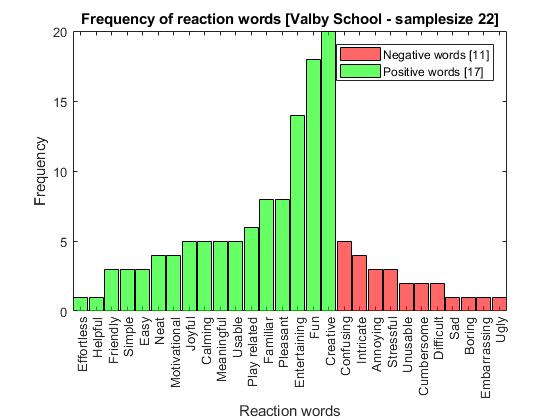
\includegraphics[width=0.7\linewidth]{figure/Evaluation/histValby.jpg}
	\label{fig:valbyTest}
	\caption{Shows frequency of selected reaction words, from the test. The bin color (red or green) divides the words in negative(red) and positive(green) }
		
\end{figure}

This suggests, that the reaction towards the usage of the tool is mostly positive.  As so, it suggests that our design requirements have been fulfilled in terms of inducing Positive emotions – in terms of a positive reaction towards the tool. However, as some negative reaction words have been selected, the deign requirement of not inducing negative emotions, cannot be stated as fully fulfilled, however as stated the overall reaction distribution suggest that, predominantly positive emotions are induced with the usage of the tool, as so, the design requirements main intentions can be said to be fulfilled. 

